\documentclass[12pt,a4paper]{report}

%Set language
\usepackage[english]{babel}
\usepackage{enumerate}

% To import and adjust images
\usepackage{graphicx}
\usepackage[export]{adjustbox}
\usepackage[center]{caption}
\usepackage{subcaption}
\usepackage{float}
\usepackage{tabularx}

% To use monospaced font
\usepackage{courier}

% To build a clickable Toc
\usepackage{color} %May be necessary if you want to color links
\usepackage{hyperref}
\hypersetup{
    colorlinks=true, %set true if you want colored links
    linktoc=all,     %set to all if you want both sections and subsections linked
    linkcolor=black,  %choose some color if you want links to stand out
    urlcolor = black
}


%To load PoLitecnico's logo
\usepackage{titling}

% Command to hide subsections in the Toc
\setcounter{tocdepth}{1}

% I don't like dots in the Toc
\usepackage{tocloft}
\renewcommand{\cftdot}{}

%To improve the tables
\usepackage[table]{xcolor}

%To break line inside tables
%\usepackage[utf8]{inputenc}
%\usepackage{fourier} 
%\usepackage{array}
\usepackage{makecell}
%\renewcommand\theadalign{bc}
%\renewcommand\theadfont{\bfseries}
\renewcommand\theadgape{\Gape[4pt]}

% Path relative to the .tex file containing the \includegraphics command
\graphicspath{ {./images/} }

% To change the ToC title
\addto\captionsenglish{ \renewcommand {\contentsname} {Table of
contents}}

%logo
\pretitle{
	 \begin{center}
	 \LARGE
	 
\includegraphics[width = 0.6\textwidth]{logo}\\[\bigskipamount]
}
\posttitle{\end{center}}

% Here we go
\title{Artificial Neural Networks and Deep Learning \\ Homework 2 - Image Segmentation, final phase}
\author{Frantuma Elia - 10567359 - 945729, \\
		Fucci Tiziano - 10524029 - 946638}
\date{A.Y. 2020/2021}

\begin{document}
	\maketitle
	%Index
	\tableofcontents
	\chapter{Introduction}
		\section{Description of the task}
			This homework consists in fine-tuning the model obtained in the Development phase. To see the model in details and its development, please follow the link in Chapter 3.

\begin{figure}[H]
\renewcommand*\thesubfigure{\arabic{subfigure}} 
\centering
\begin{subfigure}{.45\textwidth}
  \centering
  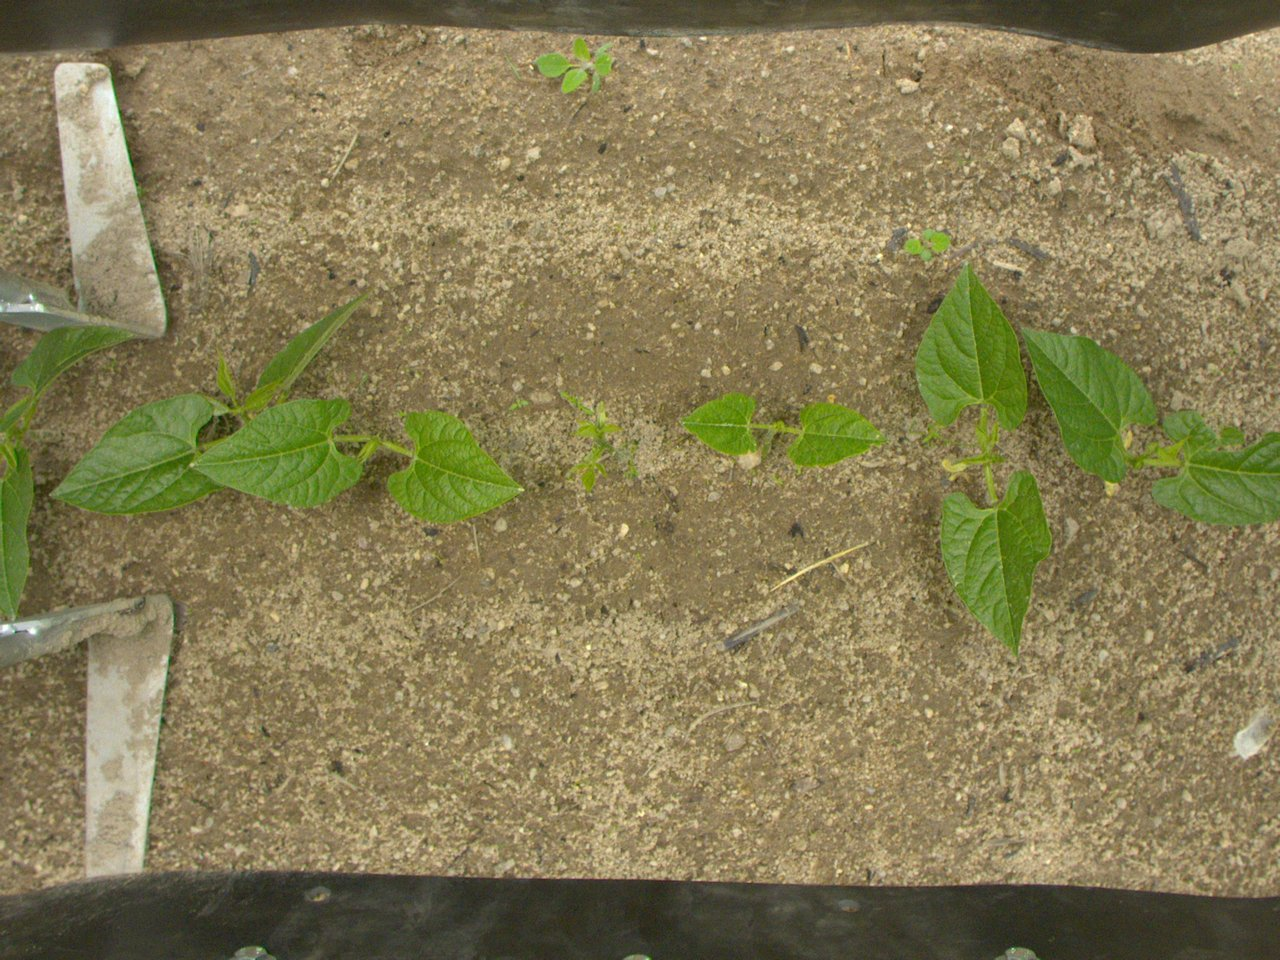
\includegraphics[width=1\linewidth]{image0}
  \caption{dataset image}
  \label{fig:sub1}
\end{subfigure}
\begin{subfigure}{.45\textwidth}
  \centering
  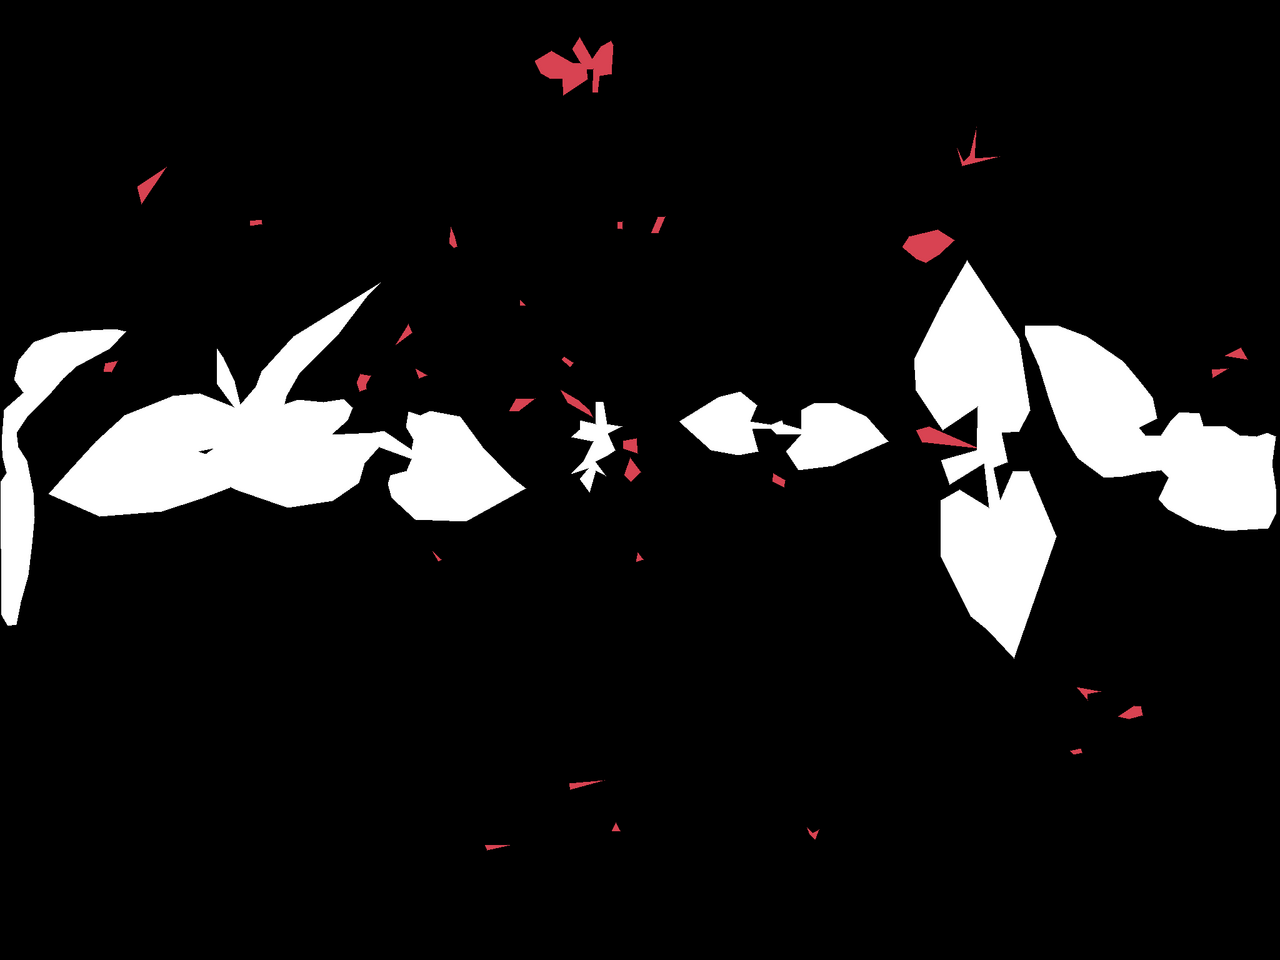
\includegraphics[width=1\linewidth]{image1}
  \caption{segmented image}
  \label{fig:sub2}
\end{subfigure}
\end{figure}

The competition is public and  organized by the ACRE (Agri-food Competition for Robot Evaluation).

	\section{Dataset}
For this final phase, the original dataset has been extended adding the Test\_Dev images. As done before, we decided to apply for maize from the Bipbip dataset.
	\subsection{Data augmentation}
We have performed data augmentation in order to increase the dataset dimension. Some of the parameters used to perform the transformations are: rotation, zoom, horizontal/vertical shift and flip.

	\subsection{Tiling}
During the training, we have experienced many issues with the RAM and VRAM. This happened both with Colab Pro and local tests. We decided not to downsize the dataset images, since the quality loss would have been too much, so we performed image tiling. In the final version, we splitted the original images into 8 tiles per image.

	\section{Validation set}

No automatic validation set is provided. This means that a subset of the training set must be used to perform validation.

In our case, we parametrized the number of training images to be moved into the validation set, with a 10\% probability.


	\section{Test set}
The test set has changed and now includes new images, which are provided without any ground-truth mask.
	\section{Evaluation}
In this final phase, there is no public evaluation. The leaderbord is published after the end of the competition.

	%end of first chapter

	\chapter{Neural network architecture}		
As in the previous phase, we have modified the function \texttt{read\_mask\_example}. The modified function can be found into the \texttt{starting\_kit} folder.
		
		\section{U-Net, with VGG as a backbone and skip connections}
The model we chose is the best performing in the Development phase.
\begin{figure}[H]
	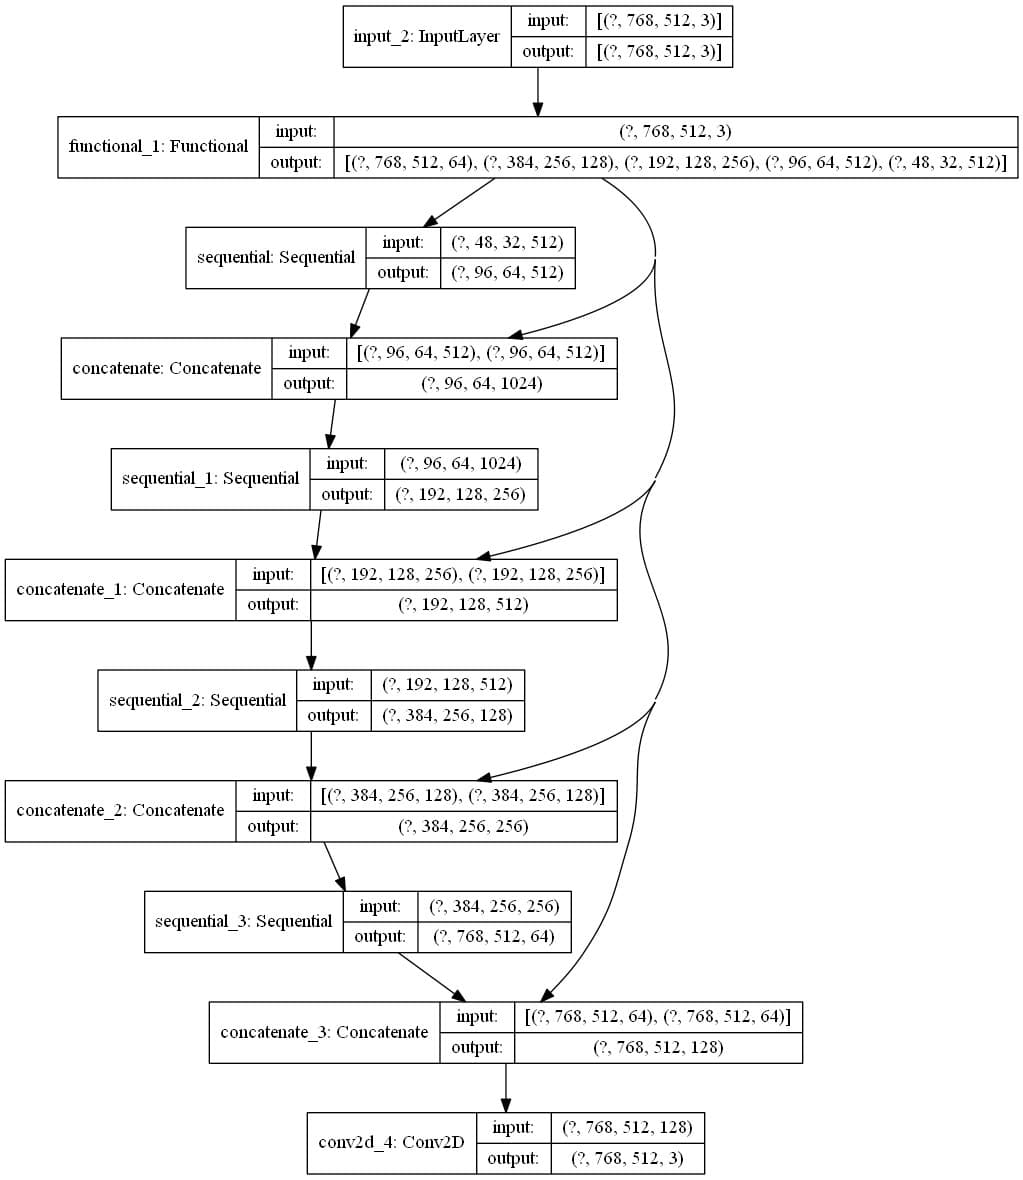
\includegraphics[scale = .45, center]{vgg_model}
	\caption{network obtained with VGG and skipped connections}
\end{figure}
\begin{figure}[H]
	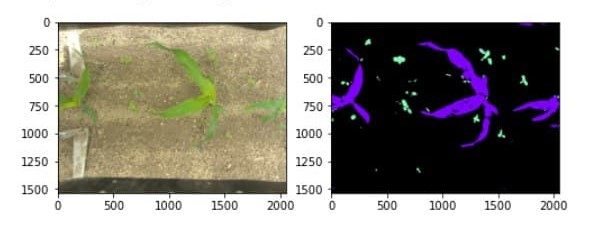
\includegraphics[scale = .75, center]{vgg_upsampling_with}
	\caption{image segmentation}
\end{figure}
		
	%end of second chapter
	\chapter{References}
		\section{Links}

\begin{itemize}
	\item GitHub repository of the project, including Development phase: \url{https://github.com/tizianofucci/A2NDLSegmentation}
	\item Competition web page: \url{https://competitions.codalab.org/competitions/27176}
\end{itemize}

\end{document}
